\documentclass[12pt, twoside]{article}
% \documentclass[12pt, twoside]{article}
\usepackage[letterpaper, margin=1in, headsep=0.2in]{geometry}
\setlength{\headheight}{0.6in}
%\usepackage[english]{babel}
\usepackage[utf8]{inputenc}
\usepackage{microtype}
\usepackage{amsmath}
\usepackage{amssymb}
%\usepackage{amsfonts}
\usepackage[nomessages]{fp} %\FPeval{\var-name}{2*sin(pi/6)}
\usepackage{siunitx} %units in math. eg 20\milli\meter
\usepackage{yhmath} % for arcs, overparenth command
\usepackage{tikz} %graphics
\usetikzlibrary{quotes, angles, arrows, arrows.meta}
\usepackage{graphicx} %consider setting \graphicspath{{images/}}
\usepackage{parskip} %no paragraph indent
\usepackage{enumitem}
\usepackage{multicol}
\usepackage{venndiagram}

\usepackage{fancyhdr}
\pagestyle{fancy}
\fancyhf{}
\renewcommand{\headrulewidth}{0pt} % disable the underline of the header
\raggedbottom
\hfuzz=2mm %suppresses overfull box warnings

\usepackage{hyperref}
\usepackage{float}

\fancyhead[LE]{\thepage}
\fancyhead[RO]{\thepage \\ First and last name: \hspace{2.5cm} \,\\ Section: \hspace{2.5cm} \,}
\fancyhead[LO]{BECA / Dr. Huson / Regents Prep: Graphs\\* 21 October 2024}

\begin{document}

\subsubsection*{1.2 Do Now: Graphing lines and finding intersections}
\begin{enumerate}
  \item Graph and label the two equations. Mark their intersection as an ordered pair.

  \begin{multicols}{2}
    $y = x-4$
    \begin{flushleft}
      Complete the table \par
      \begin{tabular}{c|c}
        $x$ & $y$ \\
          \hline
          \\
          0 & \underline{\hspace{1cm}} \\
                 \\
          2 &  \underline{\hspace{1cm}} \\
          \\
          \underline{\hspace{1cm}} & 0 \\

      \end{tabular}
      \end{flushleft}

    $\frac{1}{2}x+y = 5$
      \begin{flushleft}
      \begin{tabular}{c|c}
          $x$ & $y$ \\
          \hline
           -2 & 6 \\[5pt]
           0 & 5 \\[5pt]
           2 & 4 \\[5pt]
           6 & 2 \\[5pt]
           10 & 0 \\
          \end{tabular}
        \end{flushleft}
    \end{multicols}

  \begin{center} %4 quadrant regents grid w T-Chart
  \begin{tikzpicture}[scale=.635]
    \draw [help lines] (-10,-10) grid (10,10);
    \draw [thick, ->] (-10.2,0) -- (10.4,0) node [below right] {$x$};
    \draw [thick, ->] (0,-10.2)--(0,10.4) node [left] {$y$};
  \end{tikzpicture}
  \end{center}

\newpage
\subsubsection*{The distributive property of multiplication over addition}
\item Simplify each expression. (use fractions, not decimals)
\begin{enumerate}[itemsep=2cm]
  \begin{multicols}{2}
    \item $\frac{1}{7}+\frac{3}{7}$
    \item $4(\frac{1}{4}x + 2)$
    \item $\frac{5}{3}-\frac{1}{6}$
    \item $\frac{2}{3}(6x + 15)$
  \end{multicols}
\end{enumerate} \vspace{1cm}

\subsubsection*{Solve each equation twice, for (a) first distribute, and for (b)multiply both sides of the equation by the fraction's denominator first.}
\begin{multicols}{2}
  Distribute first \par 
  Multiply by the denominator first
\end{multicols}
\item 
  \begin{multicols}{2}
    \begin{enumerate}
      \item $\frac{1}{5}(x+8)=2$
      \item $\frac{1}{5}(x+8)=2$
    \end{enumerate}
  \end{multicols} \vspace{3cm}

\item 
  \begin{multicols}{2}
    \begin{enumerate}
      \item $\frac{1}{6}(6x+18)=11$
      \item $\frac{1}{6}(6x+18)=11$
    \end{enumerate}
  \end{multicols} \vspace{3cm}

\item Write down a rule for under what conditions is it more efficient to first distribute versus multiply by the denominator when solving an algebra equation.

\newpage
  
\end{enumerate}
\end{document}